\section{Components}

This section aims to give a short review of the main techniques and architectures used in this thesis.

\subsection{LSTM}

\begin{figure}[p]
\centering
\includegraphics[width=0.9\linewidth]{rnn}
\caption{Architecture of a vanilla recurrent neural network cell. Each timestep some output and a hidden state vector \(\mathbf{h}_t\) are produced by looking at the hidden state vector from the previous timestep \(\mathbf{h}_{t-1}\) and the current input \(\mathbf{x}_t\). In this simple example, \(\mathbf{h}_t\) is also the output.}
\label{rnn}
\end{figure}

A recurrent neural network (RNN)\cite{rnn} is a special form of neural network that is used for sequential tasks. It works by having multiple copies of the network, one for each timestep. As the input proceeds in time, each network passes information to it's next instance as seen in figure \ref{rnn}. For an input sequence \((\mathbf{x}_1, ..., \mathbf{x}_n)\) the RNN produces at each timestep \(t\) a hidden state vector \(\mathbf{h}_t\) as follows:

\begin{equation*}
  \mathbf{h}_t = \tanh \left(\mathbf{W} \begin{pmatrix} \mathbf{x}_t \\ \mathbf{h}_{t-1} \end{pmatrix} \right)
\end{equation*}

\begin{figure}[p]
\centering
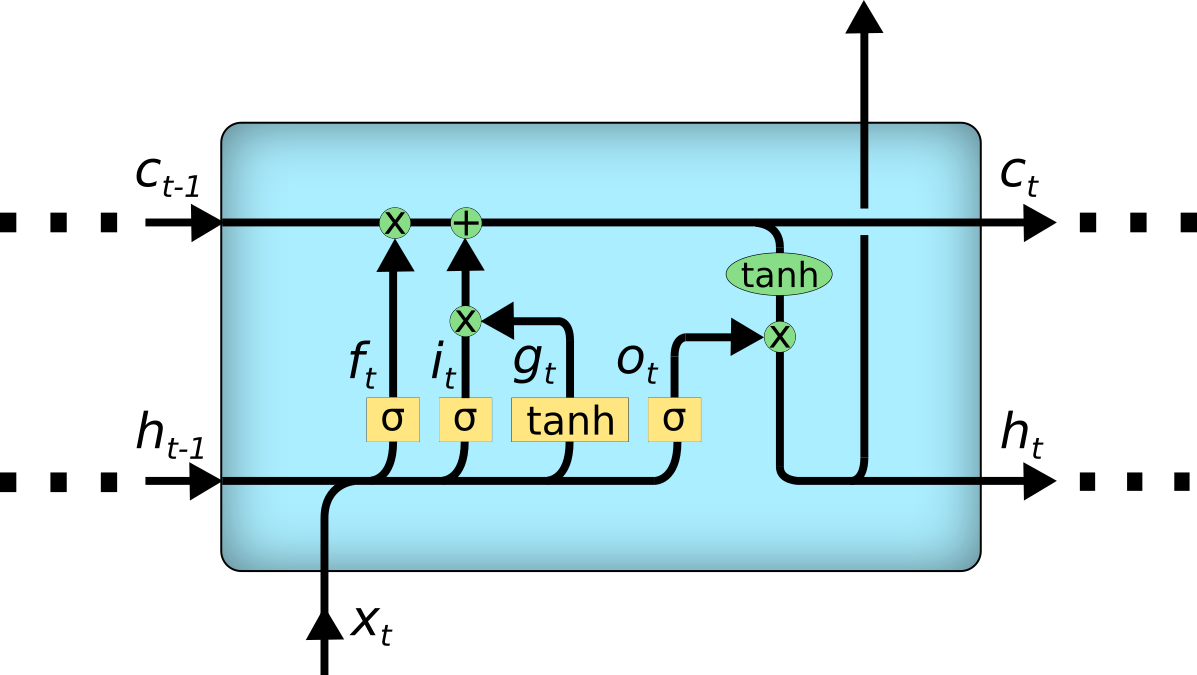
\includegraphics[width=0.9\linewidth]{lstm}
\caption{Architecture of a typical LSTM cell. In addition to the hidden state vector \(\mathbf{h}_t\), a memory state vector \(\mathbf{c}_t\) is passed to the next timestep. \(\mathbf{h}_{t-1}\) and the input \(\mathbf{x}_t\) are used to compute the gates \(\mathbf{f}_t\), \(\mathbf{i}_t\), \(\mathbf{g}_t\) and \(\mathbf{o}_t\). These gates are then used to add, delete and retrieve information to respectively from \(\mathbf{c}_{t-1}\), subsequently generating \(\mathbf{c}_t\) and \(\mathbf{h}_t\).}
\label{lstm}
\end{figure}

However, RNNs have proven to be hard to train, especially on long-range dependencies \cite{hochreiter_rnn}. In theory, they should be able to deal with these dependencies but either vanishing or exploding gradients usually prevent them from doing so. To solve this issue, Long Short-Term Memory networks (LSTMs) \cite{lstm} were proposed. In addition to \(\mathbf{h}_t\), LSTMs also pass a memory state vector \(\mathbf{c}_t\) to the next instance as can be seen in figure \ref{lstm}. The LSTM can choose at each timestep if it wants to read or forget information from the memory vector or write new information onto the vector. This is done by using explicit gating mechanisms:

\begin{align*}
  \mathbf{f}_t &= \sigma \left(\mathbf{W}_f \begin{pmatrix} \mathbf{x}_t \\ \mathbf{h}_{t-1} \end{pmatrix} \right) &
  \mathbf{i}_t &= \sigma \left(\mathbf{W}_i \begin{pmatrix} \mathbf{x}_t \\ \mathbf{h}_{t-1} \end{pmatrix} \right) \\
  \mathbf{o}_t &= \sigma \left(\mathbf{W}_o \begin{pmatrix} \mathbf{x}_t \\ \mathbf{h}_{t-1} \end{pmatrix} \right) &
  \mathbf{g}_t &= \tanh \left(\mathbf{W}_g \begin{pmatrix} \mathbf{x}_t \\ \mathbf{h}_{t-1} \end{pmatrix} \right)
\end{align*}

\noindent where \(\sigma\) is the sigmoid function. \(\mathbf{f}_t\), \(\mathbf{i}_t\) and \(\mathbf{o}_t\) can be thought of as binary gates that decide which information from \(\mathbf{c}_{t-1}\) should be deleted, which information of \(\mathbf{c}_{t-1}\) should be updated and which information from \(\mathbf{c}_t\) should be written to \(\mathbf{h}_t\).  Finally \(\mathbf{g}_t\) is a vector of possible values that (gated by \(\mathbf{i}_t\)) can be added to \(\mathbf{c}_{t-1}\) and because of the \(\tanh\) in the equation its values may range from \texttt{-1} to \texttt{1}. The state vectors are then updated as follows:

\begin{align*}
  \mathbf{c}_t &= \mathbf{f}_t \odot \mathbf{c}_{t-1} + \mathbf{i}_t \odot \mathbf{g}_t \\
  \mathbf{h}_t &= \mathbf{o}_t \odot \tanh(\mathbf{c}_t)
\end{align*}

Almost all state-of-the-art results today are achieved using either LSTMs or networks with a similar architecture like Gated Recurrent Units (GRUs) \cite{gru} because they are easier to train and excel at capturing long range dependencies.

\subsection{The Sequence-to-Sequence Model}

\begin{figure}[t]
\centering
\includegraphics[width=0.9\linewidth]{seq2seq}
\caption{The Sequence-to-Sequence Model applied to a translation example. The English source sentence is fed to the model word by word. After the input of an end-of-sequence token (\texttt{<eos>}), the network starts producing the output sentence in French. For this the produced output tokens are fed back to the network at the next timestep. The network signals the end of the sequence by outputting another \texttt{<eos>} token.}
\label{seq2seq}
\end{figure}

Traditional Deep Neural Networks (DNNs) process the whole input and then calculate some output, e.g. process an image and then classify it. This works well for problems where the input and the output are of a fixed dimension, however it is not suitable for problems where the input and the output are sequences of variable length. An example would be the input of a question and the network should produce an answer. We have seen that we can use LSTMs to process input sequences of variable length. However, in this case we want to process the whole input sequence and all the information that comes with it and only then start generating an output sequence. These problems are called sequence to sequence problems.

In \cite{seq2seq} the Sequence-to-Sequence Model is introduced as a solution to these problems. The model was applied to the task of Neural Machine Translation (NMT) and has since become the state of the art architecture in this field. The main concept can be seen in figure \ref{seq2seq}. First the whole input sequence is fed into the network and the output is ignored. Then we input an end-of-sequence token \texttt{<eos>} which signals the network to start producing the output. From there on the produced output tokens are fed to the network until the an end-of-sequence token is generated, thus signaling the end of the sequence. To speed up training the expected output is fed back to the network and not the actual produced output.

This architecture is further improved by splitting the network into two separate LSTMs. The first network takes all the input and encodes it into a vector which is then used to initialize the second network. It is first fed a start token \texttt{<GO>} and then the generated output until the end of the sequence is reached.

The network usually operates at word level and uses some word embedding like word2vec \cite{word2vec}. This method has the advantage of giving the input words some meaning through the embedding instead of just inputting a meaningless encoding of the word. While this is very effective for translation tasks, there are some limitations to this method. These embeddings work on a fixed size vocabulary which means that out of vocabulary words (OOV) can't be handled. Also special character sequences like \texttt{:)} pose a problem.

\subsection{Attention-Mechanism}

Attention is a relatively new concept for neural networks. The idea is to allow the network to chose on which information to focus at any given moment. For example in \cite{visual_attention} attention is used on the task of high resolution image classification. These kind of networks often struggle with memory constraints and attention can help them to only load the significant part of the image into the memory.

Attention has subsequently been applied to NMT \cite{attention_luong,attention_bahdanau}. The vector into which the input is encoded in the Sequence-to-Sequence model has been identified as a bottleneck which cuts down performance because of its limited capacity. After all the vector is of fixed dimensionality and needs to encode information about the whole input sequence. Because of that attention is used as a mean for the decoder to peek at previous hidden states of the encoder. This is done via a context vector \(\tilde{\mathbf{c}}_t\) which is combined with the current hidden state of the decoder \(\mathbf{h}_t\). The resulting attentional hidden state \(\tilde{\mathbf{h}}_t\) is then used by the decoder to generate the next output.

\begin{equation*}
  \tilde{\mathbf{h}}_t = \tanh \left(\mathbf{W}_c \begin{pmatrix} \tilde{\mathbf{c}}_t \\ \mathbf{h}_{t} \end{pmatrix} \right)
\end{equation*}

For the derivation of the context vector \(\tilde{\mathbf{c}}_t\) all hidden states of the encoder \(\bar{\mathbf{h}}_s\) are considered. For this an alignment vector \(\mathbf{a}_t\), whose size equals the input sequence length, is calculated from the current decoder hidden state \(\mathbf{h}_t\) and the encoder hidden states \(\bar{\mathbf{h}}_s\). The values of \(a_t\) are then normalized using the \texttt{softmax} function.

\begin{equation*}
  a_t(s) = \frac
            {\exp(\score(\mathbf{h}_t, \bar{\mathbf{h}}_s))}
            {\sum_{s'} \exp(\score(\mathbf{h}_t, \bar{\mathbf{h}}_{s'}))}
\end{equation*}

Here, \(\score\) is a content-based function used to compare the decoder hidden state \(\mathbf{h}_t\) with each of the encoder hidden states \(\bar{\mathbf{h}}_s\). There are various possible choices for this function, for example:

\begin{equation*}
  \score(\mathbf{h}_t, \bar{\mathbf{h}}_s) =
  \begin{cases}
    \mathbf{h}_t^\intercal \mathbf{W}_a \bar{\mathbf{h}}_s \\
    \mathbf{v}_a^\intercal \tanh \left(\mathbf{W}_a \begin{pmatrix} \mathbf{h}_t \\ \bar{\mathbf{h}}_s \end{pmatrix} \right)
  \end{cases}
\end{equation*}

The context vector \(\mathbf{c}_t\) is then calculated as the weighted average over the encoder hidden states.

\begin{equation*}
  \mathbf{c}_t = \sum_{s'} a_t(s') \bar{\mathbf{h}}_{s'}
\end{equation*}

\section{Dataset Construction}

For this thesis, the data from the Java Github Corpus \cite{java_dataset} was chosen. As elaborated in section \ref{code_correction_section}, a weakly typed programming language like Python would be preferable over a strongly typed one like Java because a lot of errors in Java can already be found algorithmically. However, there is a general lack of large, diverse datasets of source code thus the selection of the Java Github Corpus. Furthermore, the model knows nothing of the structure and rules of the programming language and therefore the capability of the model to grasp certain concepts can still be tested.

The Corpus was crawled from Github and includes only projects which were forked at least once to assure a certain measure of quality. It consists of around 15,000 projects which amount to approximately 15GB of data.

\subsection{Preprocessing}

Several operations were performed during preprocessing for each Java file in the dataset separately:

\begin{enumerate}
  \item All comments were removed from the file, because they are irrelevant for error detection and increase the sequence length.
  \item Line breaks were replaced by an end-of-line token.
  \item All unnecessary whitespaces were removed. This was also done to reduce sequence length because Java is a whitespace insensitive programming language, i.e. a Java program is still valid (albeit harder to understand) if its indentation is removed.
  \item If the file still contained non-ASCII characters, it was discarded. The purpose of this was to get rid of very rare characters, to reduce the input and output space and to avoid encoding errors.
  \item All method declarations were extracted from the file and checked on their corruptibility. This means, that all corruptions (see subsection \ref{corruption}) had to be able to be applied to the method.
  \item All suitable methods were then written to new files (ca. 100MB each), one method per line.
\end{enumerate}

\subsection{Corruption}
\label{corruption}

\clearpage
\thispagestyle{empty}
\begin{landscape}
  \centering
  \begin{tabular}{ | m{2cm} m{2cm}  m{8cm}  m{55mm} | }
    \hline
    Corruption & Error Type & Explanation & Example \\
    \hline
    missing bracket &
    syntax &
    A random bracket (opening or closing, regular, curved or squared) is selected and removed from the source. &
    \begin{lstlisting}
    public int add(int a, int b){
      int sum := a + b;
      return sum;
    }
    \end{lstlisting}
    \\
    missing semicolon &
    syntax &
    A random semicolon is selected and removed from the source. &
    \begin{lstlisting}
    public void add(int a, int b){
      int sum = a + b;
      return sum;
    }
    \end{lstlisting}
    \\
    misspelled variable &
    semantic &
    A random variable which is being declared in the source is selected. A random occurrence of the variable (not the one in the declaration) is then selected and misspelled. Possible misspellings are: removal of a random character, insertion of a random character, switch of two adjacent characters. &
    \begin{lstlisting}
    public int add(int a, int b){
      int sum = a - b;
      return sum;
    }
    \end{lstlisting}
    \\
    incorrect return type &
    semantic &
    The return type of the methods is changed. There are only two possibilities. If the return type is \texttt{void}, it is changed to one of Java's primitive data types (\texttt{int}, \textt{float}, etc.). In any other case, the return type is changed to \texttt{void}. &
    \begin{lstlisting}
    public int add(int a, int b){
      int sum = a - b;
      return sum;
    }
    \end{lstlisting}
    \\
    switched lines &
    logic &
    Two adjacent statement lines are switched in their order. As statement lines qualify variable declarations, assignments and method invocations. To increase the probability of an error, only lines of different types are switched. &
    \begin{lstlisting}
    public int add(int a, int b){
      int sum = a - b;
      return sum;
    }
    \end{lstlisting}
    \\
    \hline
  \end{tabular}
  \captionof{table}{Table caption}
  \label{corruption_table}
\end{landscape}

The corruption of the data was done randomly during training. 75\% of the data was left uncorrupted, meaning that the source sequence and the target sequence were identical. To the other 25\% one of five corruptions was applied, with each one being equally frequent.

Of the possible corruptions, two produced syntax errors, two semantic errors and one logic errors.

\section{Implementation}
